%
\documentclass{article}
\newcommand{\assgnnum}{2}
\newcommand{\duedate}{January 16}

\usepackage{amsmath}
%\usepackage{fullpage}
\usepackage{amssymb}
%\usepackage{bbm}
\usepackage{fancyhdr}
%\usepackage{paralist}
\usepackage{graphicx}
\usepackage{caption}
\usepackage{subcaption}
\usepackage[pdftex,colorlinks=true, urlcolor = blue]{hyperref}
\usepackage{listings}
\usepackage{color}
\usepackage{xcolor}

\definecolor{thegreen}{rgb}{0,.5,0}
\definecolor{comment-green}{rgb}{0,.3,0}
\definecolor{theblue}{rgb}{0,0,.8}
\definecolor{light-gray}{gray}{0.98}
\definecolor{comment-color}{rgb}{0,0,.8}
\definecolor{string-color}{rgb}{0,.75,0}
\definecolor{border-blue}{rgb}{0,0,.6}

\lstset{% use our version of highlighting                                            
  language=python,      % using python                                               
  keywordstyle={\color{teal}\bfseries},          % keywords                          
  commentstyle=\color{comment-color},         % comments                             
  stringstyle=\color{string-color},                   %strings                       
}

\lstset{
  basicstyle={\ttfamily\normalsize},  % use font and smaller size                    
  basewidth={0.5em,0.5em},
  showstringspaces=false,                   % do not emphasize spaces in strings     
  tabsize=2,                                % number of spaces of a TAB              
  aboveskip={0\baselineskip},               % a bit of space above                   
  columns=fixed,                            % nice spacing                           
}


\oddsidemargin 0in \evensidemargin 0in
\topmargin -0.5in \headheight 0.25in \headsep 0.25in
\textwidth 6.5in \textheight 9in
\parskip 6pt \parindent 0in \footskip 20pt

% set the header up
\fancyhead{}
\fancyhead[L]{CME193: Assignment \assgnnum}
\fancyhead[R]{Due: \duedate}
%%%%%%%%%%%%%%%%%%%%%%%%%%
\renewcommand\headrulewidth{0.4pt}
\setlength\headheight{15pt}

\newcommand{\p}{\ensuremath{\mathbf{P}}}
\renewcommand{\Pr}[1]{\ensuremath{\p \left \{ #1 \right \}}}
\newcommand{\nti}{\ensuremath{n \to \infty}}
\newcommand{\I}{\ensuremath{\operatorname{I}}}
\newcommand{\One}[1]{\ensuremath{\mathbbm{1}_{\left \{ #1 \right \}}}}
\newcommand{\E}{\ensuremath{\mathbf{E}}}
\newcommand{\Ex}[2][]{\ensuremath{\E_{#1} \left[ #2 \right]}}
\newcommand{\var}{\ensuremath{\operatorname{Var}}}
\newcommand{\cov}{\ensuremath{\operatorname{Cov}}}
\newcommand{\F}{\ensuremath{\mathcal{F}}}
\newcommand{\R}{\ensuremath{\mathbb{R}}}
\newcommand{\C}{\ensuremath{\mathbb{C}}}
\newcommand{\NormRV}[2]{\ensuremath{\operatorname{N}\left(#1, #2\right)}}
\newcommand{\BetaRV}[2]{\ensuremath{\operatorname{Beta}\left(#1, #2\right)}}
\newcommand{\argmax}{\operatornamewithlimits{argmax}}
\newcommand{\x}{\mathbf{x}}
\newcommand{\A}{\mathbf{A}}
\newcommand{\bb}{\mathbf{b}}

\newcounter{points}
\setcounter{points}{0}
\newcounter{bonuspoints}
\setcounter{bonuspoints}{0}

\newcommand\setpoints[1]{\addtocounter{points}{#1}(#1 points)}
\newcommand\setpoint{\addtocounter{points}{1}(1 point)}
\newcommand\setbonuspoints[1]{\addtocounter{bonuspoints}{#1}(#1 bonus points)}
\newcommand\setbonuspoint{\addtocounter{bonuspoints}{1}(1 bonus point)}

\newcommand\printpoints{Total number of points: \value{\thepoints}}

\newcommand{\eqD}{\ensuremath{\overset{\mathcal{D}}{=}}}

\setlength{\parindent}{0in}
\graphicspath{ {./figures/} }

\begin{document}

\pagestyle{fancy}
%\vspace*{15pt}

30 points total.  70+\% correctness (21+ points) is needed to pass.  There is also the opportunity for 4 bonus points.  Remember: you must pass all assignments to pass the class.  The assignment is due at the beginning of the next class. \\

The starter code for this assignment is available in the zip file \texttt{hw2.zip}, available on on the course web site.

\begin{enumerate}
%\item \textbf{Executing Python scripts} \\
%In Assignment 1, you used the Python interpreter.  In this assignment, you will use a text editor to write Python code in a file, or ``Python script".  You will then execute the script.  This first question is designed to make sure that everyone knows how to edit a file and execute a Python script. \\

%Open and read the file \texttt{myfirstscript.py}.  Change the value of the variable \texttt{name} to your name.  Execute the python script by typing:
%\begin{center}
%\texttt{python myfirstscript.py}
%\end{center}
%into the command line (you must be in the same directory as the script).  Alternatively, you can run the script in an integrated development environment (IDE), for example, Eclipse with the PyDev add-on.  What gets printed?  It should be something about your name and the value of pi.  Add a comment to the script saying what gets printed.  \setpoints{2}

%\newpage

\item \textbf{Coordinate systems in three-dimensions} \\
In class, we saw how to use a dictionary to store cartesian and spherical coordinates.  In this homework assignment, we will write code that converts data types between different three-dimensional coordinates systems.  First, we will review three coordinate systems.

The first system is the familiar cartesian coordinate system.  Three points, call them $x$, $y$, and $z$, are used to represent the point on three orthogonal coordinate axes.

The second system is spherical coordinates, which represents a point by a nonnegative radial distance $r$, an an inclination angle $\theta$, and an azimuthal angle $\phi$.  ($r$, $\theta$, $\phi$) represent a point on a sphere centered at the origin.  The two-dimensional analog to spherical coordinates is polar coordinates, and hence spherical coordinates are sometimes referred to as polar coordinates.  See Fig.~\ref{fig:spherical_coords} for the relationship between spherical and cartesian coordinates.

The third system is cylindrical coordinates, which represents a point by a nonnegative radial distance $\rho$, an angle $\phi$, and a height $z$.  $(\rho, \phi, z)$ represents a point on a cylinder centered at the origin.  See Fig. ~\ref{fig:cylindrical_coords} for the relationship between cylindrical and cartesian coordinates.

\begin{figure}[h!!!]
        \centering
        \begin{subfigure}[b]{0.48\textwidth}
        \centering
        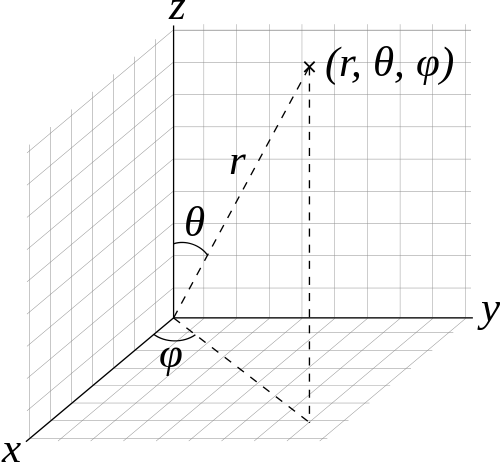
\includegraphics[height=2.9in, natwidth=610,natheight=642]{spherical}
        \caption{Spherical coordinates}
        \label{fig:spherical_coords}
        \end{subfigure}
        \quad%add desired spacing between images, e. g. ~, \quad, \qquad etc. 
          %(or a blank line to force the subfigure onto a new line)
        \begin{subfigure}[b]{0.48\textwidth}
        \centering
        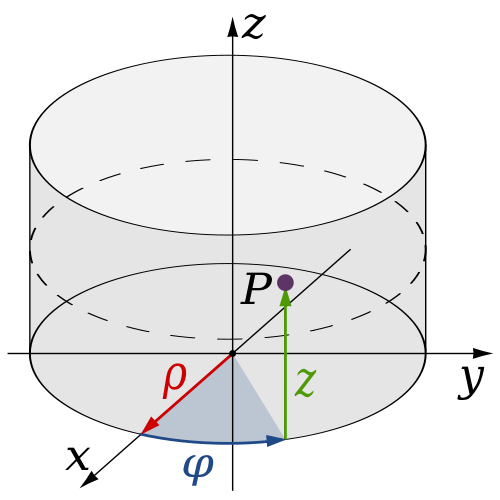
\includegraphics[height=2.9in, natwidth=610,natheight=642]{cylindrical}
        \caption{Cylindrical coordinates}
        \label{fig:cylindrical_coords}
        \end{subfigure}
         \caption{}\label{fig:coord_systems}
\end{figure}

\newpage
We will use the following formulas to convert between coordinate systems in this assignment:

\begin{itemize}
\item{cartesian $\rightarrow$ spherical: ($r = \sqrt{x^2 + y^2 + z^2}$, $\theta = \cos^{-1}\left(\frac{z}{r}\right)$, $\phi = \tan^{-1}\left(\frac{y}{x}\right)$)}
\item{spherical $\rightarrow$ cartesian: ($x = r\sin\theta\cos\phi$, $y = r\sin\theta\sin\phi$, $z = r\cos\theta$)}
\item{cartesian $\rightarrow$ cylindrical: ($\rho = \sqrt{x^2 + y^2}$, $\phi = \tan^{-1}\left(\frac{y}{x}\right)$, $z = z$)}
\item{cylindrical $\rightarrow$ cartesian: ($x = \rho\cos\phi$, $y = \rho\sin\phi$, $z = z$)}
\item{spherical $\rightarrow$ cylindrical: spherical $\rightarrow$ cartesian $\rightarrow$ cylindrical}
\item{cylindrical $\rightarrow$ spherical: cylindrical $\rightarrow$ cartesian $\rightarrow$ spherical}
\end{itemize}

where the last two conversions are compositions of the other conversions.

\begin{enumerate}
\item Finish the implementation of the functions \texttt{cart2cyl()}, \texttt{sphere2cart()}, \texttt{sphere2cyl()}, \texttt{cyl2cart()}, and \texttt{cyl2sphere()} in the file \texttt{coordinates\_tuples.py}.  The function \texttt{cart2sphere()} has already been implemented for you.  These functions convert between the coordinate systems by representing points as Python tuples in $(x, y, z)$, $(r, \theta, \phi)$, or $(\rho, \theta, \phi)$ form. Remember to use your other functions to implement \texttt{sphere2cyl()} and \texttt{cyl2sphere()}. \\

For $cos^{-1}$, use \texttt{math.acos()}; for $\sin^{-1}$, use \texttt{math.asin()}; and for $\tan^{-1}$, use \texttt{math.atan2()}.  \texttt{math.atan2()} maintains the quadrant information of its two input parameters, while \texttt{math.atan()} does not.  See \url{http://docs.python.org/2/library/math.html#trigonometric-functions} for more information.  \setpoints{9}
\end{enumerate}

\begin{enumerate}
\setcounter{enumii}{1}
\item Finish the implementation of \texttt{convert\_points()} in the file \texttt{coordinates\_tuples.py}.  This function converts a list of points in one coordinate system to a list of points in another coordinate system.  The implementation has been started for you.  \setpoints{5}
\end{enumerate}

\begin{enumerate}
\setcounter{enumii}{2}
\item Repeat part (a) in the file \texttt{coordinates\_dicts.py}.  These functions use dictionaries instead of tuples to represent points.  Again, \texttt{cart2sphere()} has been implemented for you.  For $cos^{-1}$, use \texttt{math.acos()}; for $\sin^{-1}$, use \texttt{math.asin()}; and for $\tan^{-1}$, use \texttt{math.atan2()}.  \setpoints{9}
\end{enumerate}

\begin{enumerate}
\setcounter{enumii}{3}
\item Implement \texttt{detect\_type()} in the file \texttt{coordinates\_dicts.py}.  This function determines what type of coordinate system is being used based on the keys in the dictionary.  \setpoints{5} \\
\end{enumerate}

\textbf{Grading}:

To grade this question, tests will be conducted by calling the functions you implement.  Each test is worth 0 points (do not pass test) or 1 point (pass test).  There are 28 total tests.

All of the tests used for grading are distributed with the assignment.  Gaming the autograder by hard-coding the answers of the provided test functions is considered cheating and a violation of the Stanford honor code.  I will be testing your code with additional (unreleased) tests to ensure that there is no cheating.

\newpage
\item \textbf{NumPy and SciPy} \\
In the next lecture, we will start with NumPy and SciPy, the two main Python libraries for scientific computing.  For this part of the assignment, you will get introduced to these libraries.  See course website for instructions on how to install/access these libraries.

\begin{enumerate}
\item Run the \texttt{dot()} example from \url{http://www.scipy.org/Numpy_Example_List_With_Doc}.

\setpoints{0}.
\end{enumerate}

\begin{enumerate}
\setcounter{enumii}{1}
\item Run the \texttt{integrate.quad()} example from \url{http://www.scipy.org/scipy_Example_List}.

\setpoints{0}.
\end{enumerate}


\item \textbf{Generator power (bonus: instructional only - not graded)} \\
In this bonus question, we explore generator functions.  Consider the following function, which takes as input a set of x coordinates, y coordinates, and z coordinates and returns all possible (x, y, z) points from the sets:

\begin{tabular}{c}
\lstinputlisting{code/triples.py}
\end{tabular}

\begin{enumerate}
\item
Describe a potential memory hazard with this function.  \\
\end{enumerate}

In Python, we can alternatively choose to ``yield" a value.  This allows us to iterate over objects without constructing the entire object.  These types of functions are called generating functions.  For example, the following function is the generator analog to \texttt{triples()}:

\begin{tabular}{c}
\lstset{morekeywords={yield}}
\lstinputlisting{code/triples_gen.py}
\end{tabular}

\begin{enumerate}
\setcounter{enumii}{1}
\item
What gets printed with the following code?  Explain. 

\begin{tabular}{c}
\lstinputlisting{code/triples_test.py}
\end{tabular}
\end{enumerate}

\begin{enumerate}
\setcounter{enumii}{2}
\item
Write a function \texttt{keyvals}, which takes as input a dictionary and returns a list of (key, value) tuples of all key-value pairs in the dictionary.
\end{enumerate}

\begin{enumerate}
\setcounter{enumii}{3}
\item
Write a function \texttt{keyvals\_gen}, which is the generator function analog of \texttt{keyvals} from part (c).
\end{enumerate}

\end{enumerate}
%\printpoints.
\end{document} 
